\documentclass[11pt]{article}
\usepackage[margin=1in]{geometry}
\usepackage{amsmath,amssymb}
\usepackage{graphicx}
\usepackage{listings}
\usepackage{xcolor}
\usepackage{hyperref}
\usepackage{tikz}
\usetikzlibrary{arrows.meta,shapes.geometric,positioning}

% Bitcoin-style: simple, clean formatting
\setlength{\parindent}{0pt}
\setlength{\parskip}{6pt}

% Code listing style
\definecolor{codebg}{rgb}{0.95,0.95,0.95}
\definecolor{codegreen}{rgb}{0.2,0.5,0.2}
\definecolor{codegray}{rgb}{0.5,0.5,0.5}
\definecolor{codepurple}{rgb}{0.5,0,0.5}

\lstdefinelanguage{HQL}{
  keywords={fn, const, let, var, if, cond, else, do, loop, recur, while, for, repeat, class, enum, case, new, macro, import, export, from, async, await, try, catch, finally, throw, cons, first, rest, map, filter, reduce, take, drop, range, true, false, nil, null, undefined, constructor, this, when, return},
  sensitive=true,
  morecomment=[l]{;},
  morecomment=[l]{;;},
  morestring=[b]",
  morestring=[b]',
}

\lstset{
  language=HQL,
  backgroundcolor=\color{codebg},
  basicstyle=\ttfamily\small,
  keywordstyle=\color{codepurple}\bfseries,
  commentstyle=\color{codegreen}\itshape,
  stringstyle=\color{blue},
  numbers=none,
  frame=single,
  framerule=0.5pt,
  breaklines=true,
  captionpos=b,
  tabsize=2,
  showstringspaces=false,
}

\title{\textbf{HQL: A Homoiconic Query Language}\\[0.5em]
\large A Lisp Dialect Transpiling to JavaScript}

\author{
HQL Development Team\\
\texttt{https://github.com/halcyon-lang/hql}
}

\date{}

\begin{document}

\maketitle

\begin{abstract}
\noindent A modern Lisp dialect targeting JavaScript enables functional programming with homoiconic syntax, compile-time macros, and lazy evaluation on any JavaScript runtime. HQL implements a minimal core of primitives---\texttt{quote}, \texttt{if}, \texttt{const}, \texttt{let}, \texttt{var}, \texttt{loop}, \texttt{recur}, \texttt{do}, \texttt{class}---upon which higher-level constructs are defined as macros. The transpiler converts S-expressions through a multi-stage pipeline producing zero-dependency JavaScript. JavaScript-compatible syntax for data structures and operators reduces cognitive load while preserving Lisp's metaprogramming power. A Clojure-compatible lazy sequence library provides composable data transformations. The result is a language combining Lisp expressiveness with JavaScript deployment ubiquity.
\end{abstract}

\section{Introduction}

Programming languages face a fundamental tension: expressiveness versus deployment. Lisp offers unmatched metaprogramming through homoiconicity---code as data---but historically requires specialized runtimes. JavaScript runs everywhere but lacks syntactic abstraction.

We propose HQL, a Lisp dialect that transpiles to self-contained JavaScript. The design philosophy follows three principles:

\begin{enumerate}
\item \textbf{JavaScript semantics}: Binding forms (\texttt{const}, \texttt{let}, \texttt{var}) and operators (\texttt{===}, \texttt{\&\&}, \texttt{?}) mirror JavaScript directly, reducing the learning curve.
\item \textbf{Lisp syntax}: S-expressions provide homoiconicity enabling powerful macros.
\item \textbf{Zero dependencies}: Output is a single JavaScript file with no external imports.
\end{enumerate}

\section{S-Expression Syntax}

HQL uses S-expressions as its fundamental syntax unit. Every expression is either an atom or a list:

\begin{lstlisting}
; Atoms: literals and symbols
42                    ; number
"hello"               ; string
true false            ; boolean
nil                   ; null value
my-func               ; symbol (identifier)

; Lists: function application
(+ 1 2 3)             ; => 6
(fn add [a b] (+ a b))
(if (> x 0) "pos" "neg")
\end{lstlisting}

Homoiconicity means the abstract syntax tree is directly representable in the language. This enables macros to manipulate code as ordinary data structures.

\subsection{Data Structures}

HQL adopts JavaScript/JSON syntax for composite data types:

\begin{lstlisting}
; Vectors (arrays) - JSON syntax with commas
[1, 2, 3, 4, 5]

; Hash maps (objects) - JSON syntax
{"name": "Alice", "age": 30}

; Lisp-style maps also supported
{name: "Alice", age: 30}

; Hash sets - HQL extension
#[1, 2, 3]
\end{lstlisting}

Valid JSON is valid HQL for arrays and objects, enabling seamless data interchange.

\subsection{Spread Operator}

The spread operator \texttt{...} expands arrays and objects:

\begin{lstlisting}
; Array spread
(const arr [1, 2])
[...arr, 3, 4]               ; => [1, 2, 3, 4]

; Multiple spreads
(const a [1, 2])
(const b [5, 6])
[0, ...a, 3, 4, ...b]        ; => [0, 1, 2, 3, 4, 5, 6]

; Object spread
(const defaults {host: "localhost", port: 8080})
{...defaults, port: 3000}    ; => {host: "localhost", port: 3000}

; Function call spread
(fn add [x y z] (+ x y z))
(const args [1, 2, 3])
(add ...args)                ; => 6
\end{lstlisting}

\subsection{Template Literals}

ES6-style string interpolation with backticks and \texttt{\$\{\}}:

\begin{lstlisting}
(const name "Alice")
(const age 30)
`Hello, ${name}! You are ${age} years old.`

; Expressions in interpolations
`Sum: ${(+ 2 3)}`            ; => "Sum: 5"
`Double: ${(* age 2)}`       ; => "Double: 60"
\end{lstlisting}

\section{Bindings}

HQL provides three binding forms mirroring JavaScript semantics:

\subsection{Immutable Bindings (const)}

\begin{lstlisting}
(const x 10)
(const name "Alice")
(const numbers [1, 2, 3])  ; array is frozen
\end{lstlisting}

The \texttt{const} form compiles to JavaScript \texttt{const}. Reference types are automatically deep-frozen to ensure immutability.

\subsection{Mutable Bindings (let, var)}

\begin{lstlisting}
; Block-scoped mutable binding
(let counter 0)
(= counter (+ counter 1))  ; reassignment with =

; Function-scoped mutable binding
(var total 0)
(= total (+ total 10))
\end{lstlisting}

The \texttt{let} form compiles to JavaScript \texttt{let} (block-scoped). The \texttt{var} form compiles to JavaScript \texttt{var} (function-scoped). Both permit reassignment via the \texttt{=} operator.

\section{Operators}

HQL adopts JavaScript operators in prefix notation:

\subsection{Arithmetic}

\begin{lstlisting}
(+ 1 2 3)        ; => 6  (variadic)
(- 10 3)         ; => 7
(* 2 3 4)        ; => 24 (variadic)
(/ 10 2)         ; => 5
(% 17 5)         ; => 2
(** 2 3)         ; => 8  (exponentiation)
\end{lstlisting}

\subsection{Comparison and Equality}

\begin{lstlisting}
; Relational
(< 5 10)         ; => true
(> 10 5)         ; => true
(<= 10 10)       ; => true
(>= 15 10)       ; => true

; Equality (JavaScript semantics)
(=== 1 1)        ; => true (strict)
(== 1 "1")       ; => true (loose)
(!== 1 2)        ; => true (strict)
(!= 10 20)       ; => true (loose)
\end{lstlisting}

\subsection{Logical}

\begin{lstlisting}
(&& true true)   ; => true (AND)
(|| false true)  ; => true (OR)
(! false)        ; => true (NOT)
(?? null 42)     ; => 42   (nullish coalescing)
\end{lstlisting}

\subsection{Bitwise}

\begin{lstlisting}
(& 5 3)          ; => 1  (AND)
(| 5 3)          ; => 7  (OR)
(^ 5 3)          ; => 6  (XOR)
(~ 5)            ; => -6 (NOT)
(<< 5 2)         ; => 20 (left shift)
(>> 20 2)        ; => 5  (right shift)
\end{lstlisting}

\subsection{Type Operators}

\begin{lstlisting}
(typeof 123)               ; => "number"
(instanceof arr js/Array)  ; => true
(in "x" obj)               ; => true/false
(delete obj.x)             ; remove property
\end{lstlisting}

JavaScript globals use the \texttt{js/} prefix: \texttt{js/Array}, \texttt{js/Object}, \texttt{js/Math}.

\section{Functions}

\subsection{Definition}

Functions are defined with \texttt{fn}. HQL supports exactly \textbf{two parameter styles}:

\begin{lstlisting}
; Style 1: Positional parameters with []
(fn add [a b]
  (+ a b))

; Style 2: Map parameters with {} (requires defaults)
(fn greet {name: "World"}
  (+ "Hello, " name))
\end{lstlisting}

\textbf{Important:} Parentheses-style parameters \texttt{(fn name (x y) ...)} are \textbf{NOT supported}. Only \texttt{[]} and \texttt{\{\}} are valid.

\subsection{Parameter Styles}

\textbf{Style 1: Positional parameters} use square brackets:

\begin{lstlisting}
(fn add [a b] (+ a b))
(add 5 3)                    ; => 8

; Anonymous function
(fn [x] (* x 2))

; Empty parameters
(fn get-value [] 42)

; With destructuring
(fn process [[a b] c] (+ a b c))
\end{lstlisting}

Positional parameters do \textbf{not} support default values.

\textbf{Style 2: Map parameters} use curly braces with required defaults:

\begin{lstlisting}
; Lisp style (preferred) - no commas, unquoted keys
(fn connect {host: "localhost" port: 8080 ssl: false}
  (+ (if ssl "https" "http") "://" host ":" port))

; JSON style (also supported) - commas, quoted keys
(fn connect {"host": "localhost", "port": 8080, "ssl": false}
  (+ (if ssl "https" "http") "://" host ":" port))

; Calling with partial overrides
(connect)                    ; => "http://localhost:8080"
(connect {port: 3000})       ; => "http://localhost:3000"
(connect {host: "api.com" ssl: true})
\end{lstlisting}

\subsection{Variadic Functions}

Rest parameters collect remaining arguments:

\begin{lstlisting}
; Lisp-style rest with &
(fn sum [x y & rest]
  (reduce + (+ x y) rest))

(sum 1 2 3 4 5)              ; => 15

; Rest-only
(fn log-all [& messages]
  (console.log messages))
\end{lstlisting}

\subsection{Async Functions}

Async functions use the \texttt{async} prefix:

\begin{lstlisting}
; Async with positional params
(async fn fetch-data [url]
  (const response (await (js/fetch url)))
  (await (.json response)))

; Async with map params
(async fn fetch-with-options {url: "" timeout: 5000}
  (await (js/fetch url)))

; Async anonymous
(let fetcher (async fn [url] (await (js/fetch url))))
\end{lstlisting}

\subsection{Arrow Lambdas}

Swift-inspired shorthand with implicit parameters:

\begin{lstlisting}
; Implicit parameters ($0, $1, $2...)
(map (=> (* $0 2)) [1, 2, 3])      ; => [2, 4, 6]
(filter (=> (> $0 5)) numbers)
(reduce (=> (+ $0 $1)) 0 nums)

; Explicit parameters
(map (=> [x] (* x x)) [1, 2, 3])   ; => [1, 4, 9]
((=> [x y] (+ x y)) 5 7)           ; => 12

; Property access
(map (=> $0.name) users)
\end{lstlisting}

The \texttt{\$0}, \texttt{\$1}, etc. refer to positional arguments.

\section{Control Flow}

\subsection{Conditional}

The \texttt{if} form evaluates one of two branches:

\begin{lstlisting}
(if (> x 10) "large" "small")
\end{lstlisting}

Multi-way conditionals use \texttt{cond}:

\begin{lstlisting}
(cond
  ((< x 0) "negative")
  ((=== x 0) "zero")
  (else "positive"))
\end{lstlisting}

The ternary operator \texttt{?} provides JavaScript-style conditionals:

\begin{lstlisting}
(? (> score 90) "A" "B")
(+ 10 (? true 5 3))     ; => 15
\end{lstlisting}

\subsection{Iteration}

The fundamental iteration primitive is \texttt{loop}/\texttt{recur}:

\begin{lstlisting}
(loop (i 0, sum 0)
  (if (> i 10)
    sum
    (recur (+ i 1) (+ sum i))))
\end{lstlisting}

\texttt{recur} provides explicit tail recursion, compiled to JavaScript loops.

Higher-level constructs are macros:

\begin{lstlisting}
; For loop - positional form
(for (i 5)
  (print i))           ; 0 to 4

(for (i 0 10 2)
  (print i))           ; 0, 2, 4, 6, 8

; For loop - named parameters
(for (i from: 0 to: 10 by: 2)
  (print i))

; While loop
(while (< x 100)
  (= x (* x 2)))

; Dotimes loop (executes body n times, Clojure-style)
(dotimes 3
  (print "Hello!"))
\end{lstlisting}

\section{Macro System}

The macro system enables compile-time code transformation.

\subsection{Definition}

\begin{lstlisting}
(macro when [test & body]
  `(if ~test (do ~@body)))
\end{lstlisting}

The quasiquote (\texttt{`}) templates code. Unquote (\texttt{\~{}}) evaluates expressions within templates. Splice-unquote (\texttt{\~{}@}) flattens lists.

\subsection{Expansion}

Given:

\begin{lstlisting}
(when (> x 10)
  (print "large")
  (process x))
\end{lstlisting}

The macro expands to:

\begin{lstlisting}
(if (> x 10)
  (do
    (print "large")
    (process x)))
\end{lstlisting}

\subsection{Fixed-Point Iteration}

HQL expands macros through fixed-point iteration: repeatedly apply all macros until the code stabilizes. This handles nested and mutually-recursive macro applications.

\begin{figure}[h]
\centering
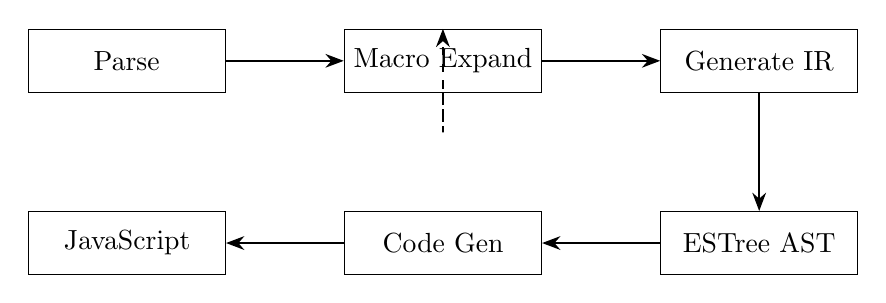
\begin{tikzpicture}[
  node distance=1.5cm,
  box/.style={rectangle, draw, minimum width=2.5cm, minimum height=0.8cm, align=center},
  arrow/.style={-{Stealth}, thick}
]
  \node[box] (parse) {Parse};
  \node[box, right=of parse] (expand) {Macro Expand};
  \node[box, right=of expand] (ir) {Generate IR};
  \node[box, below=of ir] (estree) {ESTree AST};
  \node[box, left=of estree] (codegen) {Code Gen};
  \node[box, left=of codegen] (output) {JavaScript};

  \draw[arrow] (parse) -- (expand);
  \draw[arrow] (expand) -- (ir);
  \draw[arrow] (ir) -- (estree);
  \draw[arrow] (estree) -- (codegen);
  \draw[arrow] (codegen) -- (output);

  \draw[arrow, dashed] (expand.south) -- ++(0,-0.5) -| (expand.north);
\end{tikzpicture}
\caption{Transpilation pipeline with iterative macro expansion}
\end{figure}

\subsection{Hygiene}

Manual hygiene uses \texttt{gensym} to generate unique symbols:

\begin{lstlisting}
(macro with-temp [& body]
  (const tmp (gensym "tmp"))
  `(const ~tmp nil ~@body))
\end{lstlisting}

\section{Lazy Sequences}

HQL includes a Clojure-compatible lazy sequence library, auto-loaded without imports.

\subsection{Core Operations}

The Lisp trinity of list processing:

\begin{lstlisting}
(first [1, 2, 3])      ; => 1
(rest [1, 2, 3])       ; => (2 3)
(cons 0 [1, 2, 3])     ; => (0 1 2 3)
\end{lstlisting}

\subsection{Lazy Transformations}

Sequences compute elements on demand:

\begin{lstlisting}
(take 5 (range 1000000))  ; only computes 5
(take 10 (filter (=> (=== (% $0 2) 1)) (range)))
\end{lstlisting}

Supported operations: \texttt{map}, \texttt{filter}, \texttt{take}, \texttt{drop}, \texttt{concat}, \texttt{flatten}, \texttt{distinct}, \texttt{range}.

\subsection{Eager Operations}

Reduction forces evaluation:

\begin{lstlisting}
(reduce + 0 (range 100))  ; => 4950
\end{lstlisting}

\section{Classes}

HQL supports class-based object orientation:

\begin{lstlisting}
(class Counter
  (var count 0)

  (constructor [initial]
    (do (= this.count initial) this))

  (fn increment []
    (= this.count (+ this.count 1)))

  (fn get [] this.count))

(const c (new Counter 10))
(c.increment)
(c.get)                   ; => 11
\end{lstlisting}

Classes compile directly to JavaScript classes with no runtime overhead.

\section{Enumerations}

Type-safe enumerations define named constants:

\begin{lstlisting}
; Simple enum
(enum OsType
  (case macOS)
  (case windows)
  (case linux))

; Enum with raw values
(enum StatusCodes
  (case ok 200)
  (case notFound 404)
  (case serverError 500))

; Usage
(const currentOS OsType.macOS)
(if (=== currentOS OsType.linux)
  (print "Linux!"))
\end{lstlisting}

Enums are implemented as a core compiler feature enabling IDE autocompletion via dot notation.

\section{JavaScript Interoperability}

\subsection{Method Calls}

\begin{lstlisting}
(js-call str "toUpperCase")
(js-call arr "filter" predicate)
\end{lstlisting}

Dot notation provides syntactic sugar:

\begin{lstlisting}
(str .toUpperCase)
(arr .filter predicate)
(text .trim .split " ")
\end{lstlisting}

\subsection{Property Access}

\begin{lstlisting}
(js-get obj "property")
(js-set obj "key" value)
\end{lstlisting}

\subsection{Construction}

\begin{lstlisting}
(js-new Date)
(js-new Array 10)
\end{lstlisting}

\subsection{Async/Await}

\begin{lstlisting}
(async fn fetch-data [url]
  (const response (await (js-call fetch url)))
  (await (response .json)))
\end{lstlisting}

\subsection{Error Handling}

\begin{lstlisting}
(try
  (risky-operation)
  (catch e
    (handle-error e))
  (finally
    (cleanup)))
\end{lstlisting}

\section{Module System}

\subsection{Imports}

\begin{lstlisting}
; Named imports
(import [add, multiply] from "./math.hql")

; Namespace import
(import math from "./math.hql")

; External modules
(import axios from "npm:axios")
(import fs from "node:fs")
\end{lstlisting}

\subsection{Exports}

\begin{lstlisting}
(fn add [x y] (+ x y))
(fn multiply [x y] (* x y))
(export [add, multiply])
\end{lstlisting}

The bundler inlines all dependencies into a single JavaScript file.

\section{Transpilation}

The transpiler implements a six-stage pipeline:

\begin{enumerate}
\item \textbf{Parsing}: Tokenize source into S-expression tree
\item \textbf{Import Resolution}: Load and process module dependencies
\item \textbf{Macro Expansion}: Fixed-point iteration until stable
\item \textbf{IR Generation}: Convert to JavaScript-oriented intermediate representation
\item \textbf{ESTree Generation}: Produce standard JavaScript AST
\item \textbf{Code Generation}: Emit readable JavaScript
\end{enumerate}

\subsection{Output Characteristics}

Generated JavaScript:
\begin{itemize}
\item Contains no external imports
\item Readable and debuggable
\item Compatible with Deno, Node.js, and browsers
\item Single file deployment
\end{itemize}

\section{Standard Library}

Over 40 functions load automatically:

\begin{table}[h]
\centering
\begin{tabular}{ll}
\textbf{Category} & \textbf{Functions} \\
\hline
Sequence & \texttt{first}, \texttt{rest}, \texttt{cons}, \texttt{take}, \texttt{drop} \\
Transform & \texttt{map}, \texttt{filter}, \texttt{reduce}, \texttt{flatten} \\
Generate & \texttt{range}, \texttt{iterate}, \texttt{repeat}, \texttt{concat} \\
Utility & \texttt{count}, \texttt{nth}, \texttt{last}, \texttt{distinct} \\
Map Ops & \texttt{assoc}, \texttt{dissoc}, \texttt{merge}, \texttt{keys}, \texttt{vals} \\
Higher-Order & \texttt{comp}, \texttt{partial}, \texttt{apply}, \texttt{groupBy} \\
\end{tabular}
\end{table}

\section{Implementation Status}

The implementation achieves:

\begin{itemize}
\item 89/89 language features (100\%)
\item 1457/1457 tests passing (100\%)
\item 0 type errors in transpiler
\item 68 test files covering all constructs
\end{itemize}

\section{Comparison}

\begin{table}[h]
\centering
\begin{tabular}{lccc}
 & \textbf{HQL} & \textbf{Clojure} & \textbf{Scheme} \\
\hline
Runtime & JavaScript & JVM & Native/VM \\
Bindings & JS semantics & Lisp semantics & Lisp semantics \\
Macros & Quasiquote & Quasiquote & syntax-rules \\
Lazy Seq & Yes & Yes & No \\
Output & Single JS & JAR & Implementation \\
\end{tabular}
\end{table}

HQL uniquely combines JavaScript familiarity with Lisp metaprogramming.

\section{Conclusion}

HQL demonstrates that Lisp metaprogramming is achievable on JavaScript without runtime penalty. The design choice to adopt JavaScript semantics for bindings and operators---\texttt{const}/\texttt{let}/\texttt{var}, \texttt{===}/\texttt{\&\&}/\texttt{?}---reduces cognitive load for JavaScript developers while preserving Lisp's syntactic abstraction through macros.

The language is suitable for:
\begin{itemize}
\item Educational study of Lisp and compilers
\item Rapid functional prototyping
\item Cross-platform JavaScript development
\item Metaprogramming research
\end{itemize}

Source code is available at \url{https://github.com/halcyon-lang/hql}.

\begin{thebibliography}{9}

\bibitem{mccarthy1960}
J. McCarthy,
``Recursive Functions of Symbolic Expressions and Their Computation by Machine, Part I,''
\textit{Communications of the ACM}, 1960.

\bibitem{steele1990}
G. L. Steele Jr.,
\textit{Common Lisp the Language}, 2nd ed.,
Digital Press, 1990.

\bibitem{hickey2008}
R. Hickey,
``The Clojure Programming Language,''
\textit{DLS '08}, 2008.

\bibitem{r7rs}
A. Shinn, J. Cowan, A. A. Gleckler (eds.),
``Revised$^7$ Report on the Algorithmic Language Scheme,''
2013.

\bibitem{ecma262}
ECMA International,
``ECMAScript 2023 Language Specification,''
ECMA-262, 14th ed., 2023.

\bibitem{kohlbecker1986}
E. Kohlbecker, D. P. Friedman, M. Felleisen, B. Duba,
``Hygienic Macro Expansion,''
\textit{LFP '86}, 1986.

\end{thebibliography}

\appendix

\section{Grammar}

HQL grammar in extended BNF:

\begin{lstlisting}[language={},basicstyle=\ttfamily\footnotesize]
program     = expr*
expr        = atom | list | vector | map | set
atom        = number | string | symbol | boolean | nil

list        = "(" expr* ")"
vector      = "[" (expr ("," expr)*)? "]"
map         = "{" (pair ("," pair)*)? "}"
set         = "#[" (expr ("," expr)*)? "]"
pair        = (symbol | string) ":" expr

number      = ["-"] digit+ ["." digit+]
string      = '"' char* '"'
symbol      = (letter | special) (letter | digit | special)*
boolean     = "true" | "false"
nil         = "nil" | "null" | "undefined"
\end{lstlisting}

\section{Kernel Primitives}

The kernel consists of special forms handled directly by the transpiler:

\begin{enumerate}
\item \textbf{Quoting}: \texttt{quote}, \texttt{quasiquote}, \texttt{unquote}, \texttt{unquote-splicing}
\item \textbf{Conditional}: \texttt{if}
\item \textbf{Bindings}: \texttt{const}, \texttt{let}, \texttt{var}
\item \textbf{Iteration}: \texttt{loop}, \texttt{recur}
\item \textbf{Blocks}: \texttt{do}, \texttt{return}
\item \textbf{Functions}: \texttt{fn}, \texttt{macro}
\item \textbf{Classes}: \texttt{class}, \texttt{enum}
\item \textbf{Async}: \texttt{async}, \texttt{await}
\item \textbf{Errors}: \texttt{try}, \texttt{catch}, \texttt{finally}, \texttt{throw}
\item \textbf{Modules}: \texttt{import}, \texttt{export}
\end{enumerate}

Higher-level constructs---\texttt{cond}, \texttt{when}, \texttt{unless}, \texttt{for}, \texttt{while}, \texttt{repeat}---are implemented as macros expanding to these primitives.

\section{Operator Reference}

\begin{table}[h]
\centering
\begin{tabular}{lll}
\textbf{HQL} & \textbf{JavaScript} & \textbf{Category} \\
\hline
\texttt{(+ a b ...)} & \texttt{a + b + ...} & Arithmetic \\
\texttt{(- a b)} & \texttt{a - b} & Arithmetic \\
\texttt{(* a b ...)} & \texttt{a * b * ...} & Arithmetic \\
\texttt{(/ a b)} & \texttt{a / b} & Arithmetic \\
\texttt{(\% a b)} & \texttt{a \% b} & Arithmetic \\
\texttt{(** a b)} & \texttt{a ** b} & Arithmetic \\
\hline
\texttt{(=== a b)} & \texttt{a === b} & Equality \\
\texttt{(== a b)} & \texttt{a == b} & Equality \\
\texttt{(!== a b)} & \texttt{a !== b} & Equality \\
\texttt{(!= a b)} & \texttt{a != b} & Equality \\
\hline
\texttt{(\&\& a b)} & \texttt{a \&\& b} & Logical \\
\texttt{(|| a b)} & \texttt{a || b} & Logical \\
\texttt{(! a)} & \texttt{!a} & Logical \\
\texttt{(?? a b)} & \texttt{a ?? b} & Logical \\
\hline
\texttt{(? c t e)} & \texttt{c ? t : e} & Ternary \\
\texttt{(= x v)} & \texttt{x = v} & Assignment \\
\end{tabular}
\end{table}

\section{Example: Fibonacci}

Three implementations demonstrating language features:

\begin{lstlisting}
; Recursive (naive)
(fn fib [n]
  (if (<= n 1)
    n
    (+ (fib (- n 1)) (fib (- n 2)))))

; Tail-recursive (loop/recur)
(fn fib-fast [n]
  (loop (i 0, a 0, b 1)
    (if (=== i n)
      a
      (recur (+ i 1) b (+ a b)))))

; Lazy infinite sequence
(fn fibs []
  (const fib-seq (fn [a b]
    (cons a (lazy (fib-seq b (+ a b))))))
  (fib-seq 0 1))

(take 10 (fibs))  ; => (0 1 1 2 3 5 8 13 21 34)
\end{lstlisting}

\end{document}
